\documentclass[
    %draft, % Mit % kommentieren, um Bilder sichtbar zu machen und Links zu aktivieren
    pdftex,
    a4paper,
    twoside,
    parskip=half,
    numbers=noenddot,
    listof=totoc,
    bibliography=totoc,
    hyperfootnotes=false,
    english,
    openright
]{scrreprt}

\newcommand{\todo}{\textcolor{red}{TODO}}
\newcommand{\thesistitle}{\todo}
\newcommand{\thesistype}{M A S T E R \space \space T H E S I S}
\newcommand{\thesistypedesc}{Department of Electrical Engineering and Computer Science \\
    University of Kassel}
\newcommand{\thesisauthorname}{Klara Maximiliane Gutekunst}
\newcommand{\thesisauthorhomestreet}{\todo}
\newcommand{\thesisauthorhometown}{34119 Kassel}
\newcommand{\thesisauthormatrikelnumber}{35677772}
\newcommand{\thesisauthoremail}{klara.gutekunst@uni-kassel.de}
\newcommand{\thesisdepartment}{Chair Deep Semantic Learning}
\newcommand{\thesisfirstreviewer}{Prof.\ Dr.\ Martin Potthast}
\newcommand{\thesissecondreviewer}{Prof.\ Dr.\ Gerd Stumme}
\newcommand{\thesissupervisor}{\todo}
\newcommand{\thesisdate}{\today}

% Select input encoding, usually utf8 is the best choice, on windows, \usepackage[latin1]{inputenc} maybe required
\usepackage[utf8]{inputenc}
\usepackage[T1]{fontenc}
\usepackage[english]{babel}
\usepackage{csquotes}
\usepackage{xcolor}

\MakeOuterQuote{"} % Damit ist es möglich, " " zu verwenden ohne Umlaut zu erzeugen
\defaulthyphenchar=127 % Dadurch werden auch Wörter mit Bindestrich getrennt, die schon Bindestriche enthalten.

% geometry
\usepackage[bindingoffset=1cm, left=2.5cm, right=2.5cm, top=2.5cm, bottom=2.5cm]{geometry}

% Headline
\usepackage{fancyhdr}
\pagestyle{fancy}
\renewcommand{\chaptermark}[1]{\markboth{\thechapter\ #1}{}}
\lhead{\leftmark} \rhead{\thepage}
\cfoot{}
\fancypagestyle{plain}{}

\RedeclareSectionCommand[beforeskip=1.5cm,afterskip=1cm]{chapter}

% Colors
\usepackage{color}
\usepackage{colortbl}

% Tables
\usepackage{tabularx}
\usepackage{multirow}
\setlength{\tabcolsep}{4pt}

% Drawing graphs etc.
\usepackage{pgf}
\usepackage{tikz}
\usetikzlibrary{arrows,automata}

% Footnotes
\usepackage{footmisc}
\usepackage{xspace}
\newcommand{\sic}{[\acs{sic}]\xspace}

% math
\usepackage{amsmath}
\usepackage{amssymb}

\usepackage{siunitx}

% lists
\usepackage{paralist}

% Figures
\usepackage{graphicx, wrapfig}

% Hyperlinks
\usepackage[hyphens]{url}
\usepackage{hyperref}
\hypersetup{colorlinks, citecolor=black, linkcolor=black, urlcolor=black}

% Minted
\usepackage[chapter]{minted}
%\usemintedstyle{xcode}
\setminted{frame=single,tabsize=2,linenos,autogobble}

\newmintinline[code]{text}{breaklines}

\newminted[mdcodeblock]{md}{autogobble,frame=none,linenos=false,breaklines}

% list of abbreviations
\usepackage[printonlyused]{acronym}

% Set line pitch
\usepackage{setspace}
\onehalfspacing              % anderthalbzeilig (oder auch \doublespace)

%fancyBox
%\usepackage{fancybox}

% Layout corrections (Schusterjungen)
\clubpenalty = 10000
% Layout corrections (Hurenkinder)
\widowpenalty = 10000
\displaywidowpenalty = 10000

% Figures
\usepackage{caption}
\usepackage[hypcap=true,labelformat=simple]{subcaption}
\renewcommand{\thesubfigure}{(\alph{subfigure})}
\usepackage[inkscapelatex=false]{svg}

% Tables
\usepackage{booktabs}
%\usepackage[table,xcdraw]{xcolor}

% enumerate
\usepackage{enumitem}
\newlist{questions}{enumerate}{2}
\setlist[questions,1]{label=RQ\arabic*.,ref=RQ\arabic*}
\setlist{nolistsep}

% Bibliography
\usepackage[square,numbers]{natbib}
\bibliographystyle{plainnat} % or plainnat abbrvnat unsrtnat

% Frequently used column types
\newcolumntype{C}[1]{>{\centering\arraybackslash}p{#1}} % centering column type with fixed width
\newcolumntype{R}[1]{>{\raggedleft\arraybackslash}p{#1}} % right aligned column type with fixed width
\newcolumntype{L}[1]{>{\raggedright\arraybackslash}p{#1}} % left aligned column type with fixed width

% Shortcuts for referencing floats:
\newcommand{\fig}[1]{\figurename~\ref{#1}} %shortcut for a figure reference
\newcommand{\tab}[1]{Table~\ref{#1}} %shortcut for a table reference
\newcommand{\eq}[1]{(\ref{#1})} %shortcut for an equation reference
\newcommand{\lst}[1]{Listing~\ref{#1}} %shortcut for a listing reference
\newcommand{\sect}[1]{Section~\ref{#1}} %shortcut for a Section reference
\addto\extrasenglish{%
  \renewcommand{\sectionautorefname}{Section}%
  \renewcommand{\subsectionautorefname}{Subsection}%
  \renewcommand{\chapterautorefname}{Chapter}%
}

% Shortcut for terms
\newcommand{\databaseName}{Elasticsearch}
\newcommand{\flask}{Flask}
\newcommand{\angular}{Angular}
\newcommand{\infersent}{InferSent}
\newcommand{\wordcloud}{word cloud}
\newcommand{\localMaschineStats}{Apple M2 Pro MNW83D/A with 16 \ac{gb} RAM and 12 cores}
\newcommand{\slurm}{Slurm}




\begin{document}
    \pagenumbering{roman}

    % \include{titlepage}
    % \chapter*{Abstract}
\markboth{Abstract}{Abstract}

\Acl{av} seeks to determine whether two texts share the same author, a task critical for ensuring the integrity of academic submissions or online content.
Existing approaches typically exhibit poor generalisation across domains.
The \impAppr{} introduced hard negative sampling to create input-pair-specific settings to improve cross-domain generalisation. 
However, traditional sampling strategies are unable to simultaneously control for multiple confounding variables, such as genre and topic.
%, highlighting the need for improved sampling strategies.
This thesis investigates whether \aclp{llm} can help address these limitations. 
Specifically, we employ \acs{llm}-generated paraphrases as hard negatives. 
% Since these paraphrases aim to preserve the confounding variables of the original text, they mitigate domain-related biases during inference. 
% Moreover, by constructing a tailored case for each input text pair, the approach eliminates out-of-distribution issues, ensuring that comparisons remain within the distribution defined by the pair itself.
Evaluation on the \dataStudent{} dataset from the original study shows that the \acs{llm}-based extension surpasses the original baselines by \citet{koppel_determining_2014}, \acs{ppmd}, and \unmasking{} in terms of precision and recall.
At the same time, our results reveal the practical and conceptual challenges of integrating \acsp{llm} into \acl{av}, including issues of reliability, hallucination, and control over paraphrase quality.



% The original \impAppr{} compares a disputed text to a candidate text and hard negatives, considering disputed and candidate text to share an author if the candidate is consistently the most similar across random feature projections. 
    % \chapter*{Zusammenfassung}
\markboth{Zusammenfassung}{Zusammenfassung}



    \tableofcontents

    \chapter*{List of abbreviations}
\markboth{List of abbreviations}{List of abbreviations}

\begin{acronym}[XXXXXXXXX]
    \acro{ai}[AI]{Artificial Intelligence}
    \acro{ir}[IR]{Information Retrieval}
    \acro{nlp}[NLP]{Natural Language Processing}
    \acro{llm}[LLM]{Large Language Model}
    \acro{roc-auc}[ROC-AUC]{Area Under the Receiver Operating Characteristic Curve}
    \acro{pan}[PAN]{Plagiarism Analysis and Authorship Mining} % TODO: find out if correct
    \acro{bert}[BERT]{Bidirectional Encoder Representations from Transformers}
    \acro{bow}[BoW]{Bag-of-Words}

    % \acro{}[]{}
\end{acronym}


    \pagebreak
    \pagenumbering{arabic}

    % % Hier weitere Kapitel einfügen
    % \chapter{Introduction}
\label{chap:introduction}



% motivation
Historically, authorship analysis focused on literary disputes~\citep{neal_surveying_2018,stamatatos_survey_2009}, but contemporary concerns have shifted towards practical applications.
In an era where large amounts of text can be copied, paraphrased, or fabricated with ease, determining the true author of a text is crucial for maintaining trust in communication. 
Scenarios include detecting plagiarised passages of texts~\citep{stein_intrinsic_2011}, and verifying the authenticity of online content or student submissions. 
Formally, we refer to these problems as \acf{av} or \acf{aa}, where every \ac{aa} task can be formulated as a sequence of \ac{av} problems~\citep{tyo_state_2022,barlas_cross_domain_2020}.

The emergence of \acp{llm} adds an additional layer of complexity. 
While these models are widely embraced for beneficial applications such as summarisation, information seeking, and assistive writing~\citep{wang_stumbling_2024}, their ability to convincingly imitate human writing creates new risks. 
\acp{llm} can be used to generate misinformation, impair academic honesty, or impersonate individuals, thereby inflicting harm on individuals who fall victim to these schemes~\citep{mitchell_detectgpt_2023,li_learning_2025,wang_stumbling_2024,bhattacharjee_fighting_2024}. 
Since \acp{llm} can be conceptualised as authors, their detection naturally falls within the scope of \ac{av}. 
Thus, instead of treating \ac{llm} detection as an isolated task, it is more consistent to frame it as a specialised case of \ac{av}~\citep{llm_detection_av_2025}.

% specificity rather than generality
Existing approaches to generalisation typically train a single model and apply it across domains.
Despite significant advances in \ac{av}, prior work finds that such models struggle in \ac{ood} settings, where the topic or genre diverges from the training data~\citep{Sundararajan_style_18,bischoff_importance_2020,li_learning_2025}. 
This shortcoming motivates a shift towards scenario-specific solutions, i.e.\ models are trained anew for narrowly defined cases. 
Such single-case approaches enable more precise control over contextual factors and place greater emphasis on stylistic idiosyncrasies rather than domain-level variation.

% AV
The \impAppr{} by \citet{koppel_determining_2014}\ introduces the idea of generating \imp{} texts, i.e.\ hard negatives, used to sharpen the discrimination between genuine and false authorship matches. 
However, the method's effectiveness is limited by the quality and contextual adequacy of these \imp{} texts. 
Previous work did not fully address how to construct challenging \imps{} via controlled contextual variables.

The thesis extends the \impAppr{} by leveraging \acl{sota} \acp{llm} to generate paraphrases as \imps{}, enabling control over multiple confounding factors such as genre, topic, and target audience. 
In doing so, the approach shifts the focus towards authorial style rather than domain differences, yielding improved precision–recall on the \dataStudent{} dataset compared with the original sampling strategies, \unmasking{} and \acs{ppmd}.


\section{Research Questions}
\label{sec:research_questions}
To guide this objective, we formulate the following research questions:
\begin{questions}
    \item \textbf{How can we instruct a \ac{llm} to paraphrase the text of a candidate author such that it captures the \ac{llm}'s stylistic properties?} \label{enum:rq1} \hfill \\
    The goal is to create hard negatives for the Impostor method by controlling contextual factors.
    By controlling genre, topic and other factors, similarity measures primarily focus on differences in authorial style rather than the impact of content on style.
    We obtain this controlled environment by utilizing \acp{llm} to paraphrase the original text.
    There are different approaches to paraphrasing text using \acp{llm}.
    They include (a) directly asking the \ac{llm} to paraphrase the text, 
    (b) first extracting specific information from the original text and subsequently generating a paraphrase based on the information.
    This thesis compares both approaches on \dataStudent{}, \dataBlog{}, \dataGutenberg{} and \dataPan{}.

    \item \textbf{How do we evaluate the quality of paraphrases?} \label{enum:rq2} \hfill \\
    Paraphrase evaluation is inherently challenging, as there is no universally agreed-upon definition of what constitutes a paraphrase. 
    Prior research often adapts evaluation metrics from related \ac{nlp} tasks such as machine translation or summarization. 
    Two key dimensions are typically considered: semantic similarity and syntactic similarity.
    Contrary to initial intuition, high syntactic similarity is not necessarily desirable, as it may indicate that the \ac{llm} has merely copied the original text with minimal changes. 
    Instead, our focus lies on achieving high semantic similarity while maintaining syntactic diversity to ensure genuine rephrasing.
    Furthermore, we acknowledge that relatively low automatic scores can still be acceptable if qualitative human evaluation confirms the paraphrase’s adequacy.

    % \item \textbf{Which features are used for the \ac{av} problem?} \label{enum:rq3} \hfill \\
    % Traditional features include character tri-gram features, while newer research has proposed using \ac{llm} such as BERT.

    \item \textbf{How does the \ac{llm}-based impostor approach perform compared to state-of-the-art models?} \label{enum:rq4} \hfill \\
    Though our approach is computationally expensive, we argue that it is not a general purpose \ac{llm} detection method, but rather a single case solution tailored to specific detection tasks.
    We evaluate its performance in scenarios where (a) the disputed text is human generated,
    (b) the disputed text is \ac{llm} generated and the candidate is the same \ac{llm}, and
    (c) the disputed text is \ac{llm} generated, but the candidate is a different \ac{llm}.
    In terms of performance, we compare our method to other \ac{av} approaches on the \dataStudent{}, \dataBlog{}, \dataGutenberg{} and \dataPan{} datasets.
    
\end{questions}

% \section*{Idea}
% \label{sec:idea}

% Given a text of unknown authorship (i.e., human or \ac{llm}), 
% construct a set of impostor texts using state-of-the-art \acp{llm} based on the original text.
% Obtain the author by \ac{aa}/ \ac{av} methods, such as unmasking, to \textit{confidently}, i.e. high precision, identify \ac{llm} generated texts
% (and possibly which \ac{llm}).



\section{Contributions}
\label{sec:contributions}
The contributions of this thesis are:
\begin{enumerate}
    \item Reimplementation of the traditional Impostor approach (cf. \autoref{chap:implementation}).
    \item Extension of the impostor approach with \ac{llm} generated impostors for line-up of difficult opponents (cf. \autoref{chap:methodology}). 
    \item Frame \ac{llm} detection as a \ac{av} problem and use \ac{llm} generated text as candidate for text of "unknown" authorship.
\end{enumerate}


\section{Thesis Structure}
\label{sec:thesis_structure}
The thesis is structured as follows:
    % \chapter{Related Work}
\label{chap:related_work}

This work is different to the work of \citet{koppel_determining_2014} and \citet{kocher_unine_2015} 
in that it uses \acp{llm} to generate imposter texts.

% AV

% LLM detection using generative models
%% AA against LLMs
With the recent advances of \ac{nlg} come new challenges in text authorship.
The new technologies may be misused for fraudulent activities to scam naive or inexperienced users~\citep{uchendu_authorship_2020,bhattacharjee_fighting_2024}.
\citet{uchendu_authorship_2020} identified three authorship tasks essential for fighting fraudulent activities:
(1) Given two texts $t_1$ and $t_2$, determine whether they were produced by the same method (i.e. human author or a specific \ac{nlg} method).
(2) Given a text $t$, determine whether it was human authored or machine generated (Turing Test).
(3) Given a text $t$, find its author among $k+1$ candidates, which consists of one human and $k$ machines.
They compare classical \ac{ml} models, neural models and state-of-the-art \ac{aa} models as classifiers 
for these single- (Problem 1 and 2) and multi-class (Problem 3) tasks.
Their findings include, that as of 2020, most \ac{nlg} methods were distinguishable from human authors, 
but some \acp{llm} proved difficult to detect.
%%% compared to our work
In the following, we consider (1) \ac{av}, (2) classical \ac{llm} detection, and (3) closed-set \ac{aa}.
Our approach differs from the work of \citet{uchendu_authorship_2020} in that our candidates (i.e. imposters) do not include a human author (3), 
but only \acp{llm}.
Moreover, we use different classifiers originally designed for \ac{av}, rather than \ac{aa}.

%% LLM (gpt-3.5, GPT-4) as detector
\citet{bhattacharjee_fighting_2024} evaluate using an \ac{llm} as classifier for \ac{llm} detection.
They use \ac{gpt}-3.5 and \ac{gpt}-4 to classify texts as human or machine generated.
They find that \ac{gpt}-3.5 performs better when being fed simple instructions, rather than constrained prompts.
They find that \ac{gpt}-4 predicts almost exclusively \ac{ai} generated texts, 
while \ac{gpt}-3.5 predictions are more reliable (especially for actually human authored texts).
%%% compared to our work
Our work differs from theirs in that we use \acp{llm} to generate imposter texts specific to the candidate text, 
rather than using the publicly available dataset TuringBench with previously generated texts.

%% DetectGPT: Perturb (Mask), score, compare (unsupervised)
\citet{mitchell_detectgpt_2023} propose DetectGPT, a method that is threefold:
(1) They perturb the input text by (1.1) masking out random 2-word spans until 15 \% of the text is masked. 
Masked spans are replaced (1.2) with words from an off-the-shelf (i.e. not finetuned to target domain) \ac{llm} (e.g. T5-3B). 
These perturbations are semantically similar paraphrases of the original text.
(2) They score (in terms of log probability) each perturbed text using a scoring \ac{llm} 
(ideally their candidate \ac{llm}, but it works also with any \ac{llm}, though scores deteriorate). 
(3) The difference of the score of the original text and the average score of the perturbed texts is denoted perturbation discrepancy $d$. 
(4) Normalize $d$ by the standard deviation of the scores of the perturbed texts.
(5) Based on a threshold $\epsilon=0.1$, classify the original text as human authored or machine generated 
(formally Local Perturbation Discrepancy Gap hypothesis).
If $d$ is positive, the original text is likely machine generated.
If $d$ is near zero, i.e. $d < \epsilon$, the original text is likely human authored.
\citet{mitchell_detectgpt_2023} motivate their method by the observation that generated texts tend to occupy 
negative curvature regions of the model's log probability function (i.e. they lie on the local maximum of the manifold).
When the text is machine generated, it lies on a local maximum, 
and perturbing it will lead to lower log probabilities of perturbed texts.
When the text is human authored, it does not lie on a local maximum to begin with, 
rendering log probabilities of perturbed texts similar either bigger or smaller than the original text.
Averaging the log probabilities of perturbed human texts leads to a value that is 
close to the original text's log probability (i.e. a perturbation discrepancy $d$ near zero).
Even though, DetectGPT works best when the source (i.e. generating) \ac{llm} and the scoring \ac{llm} are the same 
(requires white-box access to the \ac{llm}), 
it works also with different \acp{llm} as surrogate for the source model when scoring (in a black-box case).
%%% compared to our work
We can not supply a white box setting, because we do know the source \ac{llm} that generated the imposter texts.
%%%% imposters and perturbations
However, this approach is similar to our approach, because perturbing texts can be seen as a 
form of imposter generation (especially as we use paraphrases). 
%%%% sample from the source model
Both approaches try to sample from the probability distribution of the source model either 
by using imposters (via prompting an \ac{llm}) or by perturbing the original text (using an \ac{llm}).
%%%% input
While the imposter approach is an \ac{av} task (i.e. input is a disputed and a candidate text), 
DetectGPT receives a disputed text and a candidate \ac{llm} as input.
%%%% similarity measure
While we use a similarity measure on traditional n-gram frequency vectors, 
\citet{mitchell_detectgpt_2023} require a scoring \ac{llm} to compute the perturbation discrepancy $d$.
Hence, our approach is easier in terms of computational resources and requirements.

%% LLM rewrite LLM texts less than human texts (no AA, but edit distance hypothesis)
RAIDAR~\citep{mao_raidar_2024} builds upon the invariance property of \acp{llm}, 
which states that prompting an \ac{llm} to rewrite a machine generated text will introduce little change.
They motivate this by the observation that (different) autoregressive models produce similar patterns and thus, 
consider texts generated by (different) \acp{llm} as high quality that do not require rewriting.
Change is measured by the edit distance between the original text and the rewritten text. 
\citet{mao_raidar_2024} propose using an edit distance based on the Levenshtein distance or \ac{bow} representations.
RAIDAR operates on character level rather than using deep neural network features, and it does not require the original generating model for classification. 
RAIDAR fails to detect \ac{llm} generated texts in out-of-distribution scenarios (i.e. different domains than training), 
or when \ac{llm} were explicitly instructed to produce text prone to heavy \ac{llm} modification when being asked to rewrite the text \citep{li_learning_2025}.
Based on RAIDAR (\citep{mao_raidar_2024}), \citet{li_learning_2025} propose fine-tuning an \ac{llm} to rewrite human authored texts more than machine generated text.
Classification is carried out by comparing the edit distance of the original text and the rewritten text to a threshold.
\citet{li_learning_2025} admit that their approach is slow in inference time, 
since a candidate text has to be rewritten multiple times (about 200 different prompts) to obtain a reliable score.
\citet{mao_raidar_2024} find that the quality of perturbation based models (i.e. rewriting) for \ac{llm} detection correlates with the perturbation model size.
\citet{mitchell_detectgpt_2023} find a negative correlation (\textcolor{red}{TODO: chapter 2 vorletzter Absatz}) between the size of the perturbation model and the performance of DetectGPT.
%%% compared to our work
%%%% generation of texts during inference
Both approaches are similar to our work in that they use \acp{llm} to generate texts during inference.
We do not fine-tune an \ac{llm} for paraphrasing but use off-the-shelf models (like RAIDAR).
%%%% similarity measure
All these approaches compute the similarity of the original text and the generated text.
However, we do not use edit distance (i.e. Levenshtein distance) as similarity measure.
%%%% limitations
This approach is unable to detect which \ac{llm} generated the text.

%% LLMDet: Proxy to perplexity (problem: requires access to the LLM to build the dictionary)
Perplexity is a reliable statistical metric for attributing texts to \acp{llm}~\citep{zhang_llmdet_2023}.
Unfortunately, perplexity requires access to \acp{llm}' parameters (i.e., white-box detection).
\citet{zhang_llmdet_2023} propose LLMDet, a method that uses a proxy to perplexity, 
where a dictionary of frequent n-gram (frequent among $n$ randomly prompted generated texts per \ac{llm}) 
next token probabilities is pre-computed (i.e. requiring access to the \ac{llm}), 
and is subsequently used during inference to approximate perplexity by replacing $x_{<i}$ in $p(x_i | x_{<i})$ with an n-gram.
Since the construction of the dictionary requires access to the \ac{llm}, LLMDet requires contribution of the closed-source model owners.
The disputed text is tokenized and the proxy perplexity is calculated for each model and thus, constructing a proxy perplexity vector.
This vector is input to a trained classifier.
%%% compared to our work
Proxy perplexity could be used as a baseline for our approach, though it requires access to the \ac{llm} and is thus not applicable in our case.

%% Mirror Minds: extract query, genrate two paraphrases, compare & classify via threshold (very similar to our work)
\citet{baradia_mirror_2025} propose (1) extracting a query from the disputed text, which captures the essence of the text, 
(2) generating two paraphrases of the original text using the query as input prompt to two \acp{llm}, 
and (3) comparing the paraphrases to the original text via the BLEU and the METEOR score.
Both score capture syntactic similarity, even though \citet{baradia_mirror_2025} argue they also capture semantic similarity.
They use the maximum across the two models per similarity measure as a final score pair.
Classification of the resemblance to \ac{ai} generated content requires a threshold.
%%% compared to our work
%%%% same approach
This approach is similar to our approach in that it uses \acp{llm} to generate paraphrases of the original text.
Moreover, it compares the original text to the generated paraphrases as in a \ac{aa} problem. % rather AI detection?????
%%%% similarity measure
We do not use BLEU or METEOR as similarity measure, nor do we compare directly on paraphrase-level (i.e. BLEU calculates n-gram overlap) 
but construct our own frequency based n-gram vectors input vector similarity metrics.
%%%% they discard information, solve another problem
However, this approach discards the information which \ac{llm} produced the most similar paraphrase. 
While our goal is to solve an \ac{aa} problem (i.e. multiclass classification), 
\citet{baradia_mirror_2025} solve a binary classification problem (i.e. human vs. \ac{ai} generated text).
    % \chapter{Methodology}
\label{chap:methodology}

\subsection{Dataset}
\label{subsec:dataset}

\subsubsection{Original Data}
Due to this approach extending the original imposter approach by \citet{koppel_determining_2014}, 
we first use original data to establish the feasibility and reproducibility of the original approach. 
\citet{koppel_determining_2014} used \dataBlog{} and the \dataStudent{} dataset.
The  \dataStudent{} dataset is not publicly available, due to sensible information about the students.
J. W. Pennebaker was kind enough to provide us with the original data M. Koppel used in his paper.
The dataset contains student essays for five assignments from a class in 2006.
The assignments include stream of consciousness, talk about your childhood, describe your personality, 
Thematic Apperception Test, and Give four examples of four different theories.
For reproducing our work, due to privacy concerns, 
we refer to J. W. Pennebaker as the data holder  and authority of the \dataStudent{} dataset.
For establishing a baseline for the imposter approach, we use the \dataBlog{} and the \dataStudent{} dataset.

\subsubsection{Additional Data}
To extend our test scenario for the imposter approach, we opted to find an additional dataset that fulfilled the following criteria:
\begin{itemize}
    \item controlled confounders (e.g. genre, topic)
    \item undisputed authorship 
    
\end{itemize}

We found that both the \dataPan{} and \dataGutenberg{} datasets are suitable candidates.
The statistical properties of the datasets are shown in \autoref{tab:data_stats}.

\begin{table}[h]
\centering\small
\caption{Statistics of preprocessed datasets \dataPan{}, \dataBlog{} and \dataGutenberg{}.}
\label{tab:data_stats}
\resizebox{\textwidth}{!}{%
\begin{tabular}{@{}lrrrrrrrrr@{}}   % numbers should be right aligned, text left aligned
\toprule
dataset & num\_pairs & num\_authors & num\_same\_pairs & num\_different\_pairs & avg\_text\_len & min\_text\_len & max\_text\_len & std\_text\_len & median\_text\_len \\ 
\midrule
pan20     & 66912 & 52778 & 35620 & 31292 & 21435.53  & 20670 & 296887  & 2685.49   & 21284.00  \\ 
blog      & 64771 & 18961 & 33639 & 31132 & 1846.20   & 501   & 615409  & 3461.74   & 1244.00   \\ 
gutenberg & 36    & 4     & 15    & 21    & 293840.11 & 14092 & 1176438 & 339991.16 & 139370.00 \\ 
\bottomrule
\end{tabular}%
}
\end{table}
\textcolor{red}{above len in characters, but I have also stats for words‚}


\subsubsection{Dataset Preprocessing}
\label{subsubsec:dataset_preprocessing}

To further control confounders influencing authorial style, we preprocess the dataset 
(once before creating the arrow dataset file and once before using the detector).
The requirements for the preprocessing are:
\begin{itemize}
    \item The texts are stripped of all format/ layout information to obtain plain text \textcolor{red}{TODO: before saving them as arrow files}.
    \item The texts should be of similar length (detector crops texts to the length of the shorter text).
\end{itemize}
In order to produce a controlled testing environment four our imposter approach, 
we opted to refine few datasets rather than scaling up to larger datasets.
Removing layout information includes removing HTML artefacts, play artefacts, newlines, 
converting utf-8 to ASCII, lowercasing and stripping leading and trailing whitespace.

\subsubsection{Selection of Text Pairs}
\label{subsubsec:dataset_text_pair_selection}

We had to select pairs of texts for the \dataBlog{} and the \dataGutenberg{} dataset.
We decided to keep the existing pairs in the \dataPan{} arrow dataset for better comparability.
All datasets consist of same- and different-author pairs. 
As mentioned before, we aimed to control confounders when selecting pairs.

For the \dataBlog{} dataset, 
two texts of a pair are selected such that they share the same topic, year, gender and age, where the last to reference the text's author.
Test (20\%) and train split (80\%) have different topics.

For the \dataGutenberg{} dataset,
we selected pairs of texts that share the same genre and century.
Authors can either be in the train (80\%) or test (20\%) set.

Irrespective of the information used to select pairs, the final dataset contains only the columns \texttt{authors}, \texttt{pair}, and \texttt{same}.
The \texttt{pair} column contains the texts of the pair as a list of strings,
the \texttt{authors} column contains the authors of the texts as a list of strings,
and the \texttt{same} column indicates whether the texts are from the same author (\texttt{True}) or from different authors (\texttt{False}).


\subsection{Imposter Generation}
\label{subsec:impostor_generation}

% good impostors: hard negatives
Equivalent to the original impostor approach by \citet{koppel_determining_2014}, we denote ideal impostor texts as hard negatives.
In other words, texts that are not authored by the candidate author, but are difficult to distinguish from the candidate author's texts.
Note that the quality of the impostors directly contributes to the performance of the model, 
since easy impostors lead to \acp{fp} and too difficult ones to \acp{fn}.

\subsubsection{Traditional Imposter Generation}
\label{subsubsec:traditional_impostor_generation}

To assess the quality of our Imposter approach implementation, we first reimplement the original impostor approach by \citet{koppel_determining_2014}.
The parameters are set to the original default values.


\subsubsection{Novel Imposter Generation}
\label{subsubsec:novel_impostor_generation}
% obstacles for impostor generation in the past
The traditional generation techniques outlined by \citet{koppel_determining_2014} faced difficulties in controlling essential factors such as text topic or genre.
Since authorial style heavily depends on these factors, traditional impostors can differ a lot from the candidate text.
% model process of original text generation
The ideal generation technique would model the process of the original text generation, 
i.e. among others, the author's task, and references.
Hence, all external influential factors are specified to match the original conditions.
Unfortunately, due to the nature of this task 
(i.e. requirement of \ac{av} is often linked to a lack of information of the author either due to death in the case of literary texts or 
due to unwillingness of cooperation in case of plagiarism), this information is in most cases not available.
% heuristics: paraphrase
With \acp{llm} it is possible attempt to control external factors and 
as a heuristic to modelling the generation process, paraphrase the original text.
% lack of definition of paraphrase
Due to the lack of a universal definition of paraphrases~\citep{gohsen_task_oriented_2024}, the following criteria are used to determine the quality of the generated paraphrases:
% our criteria for good paraphrases
\begin{itemize}
    \item The generated text should belong to the same topic, genre and exhibit the same tone (\textcolor{red}{=tone???}) as the original text.
    \item The semantic information may differ (i.e. hallucination is allowed).
    \item The generated text should be different to the original text in terms of style, i.e. wording and sentence structure (i.e. syntactic similarity). \textcolor{red}{threshold to exclude near-duplicate paraphrases~\citep{gohsen_captions_2023}?}
\end{itemize}


% Notes
According to \citet{gohsen_task_oriented_2024}, there are two perspectives to paraphrasing: 
Lexical (i.e. changes at word level) and syntactic (i.e. changes at syntactic level).
Paraphrase types can be classified into surface and semantic level. Finer levels are outlined in \citep{gohsen_task_oriented_2024}.

Popular paraphrase categories include \citep{fu_learning_2024}:
\begin{itemize}
    \item Top-level classification perspective: 
        \begin{itemize}
            \item Lexicon-based changes
            \item Morphology-based changes
            \item others
        \end{itemize}
    \item Second-level classification perspective:
        \begin{itemize}
            \item Change of format
            \item Semantic-based
            \item Change of order
        \end{itemize}
\end{itemize}

\citet{zhou_paraphrase_2025} (pg. 3, tab.1, and examples afterwards) define a topology of paraphrase types:
\begin{itemize}
    \item Morphology based: inflection changes (e.g. singular to plural), derivation changes (e.g. adjective to verb), functional word substitution (e.g. this to that).
    \item Lexicon based: Same polarity substitution (e.g. synonym), opposite polarity substitution (e.g. antonym), converse substitution (e.g. opposite view point), spelling changes, synthetic/ analytic substitution, relational substitution
    \item Syntax based: Negation switching (i.e. other negation), diathesis alternation (e.g. change position of verb), etc.
    \item Discourse based: Indirect/direct substitutions, sentence modality changes, punctuation changes, etc.
    \item Other changes: Change of order, change of format, etc.
\end{itemize}

\citet{zhou_paraphrase_2021} claim it is difficult to control the style of generated paraphrases.

Another approach to paraphrasing is back-translation, which may limit diversity \citep{zhou_paraphrase_2025}.


\subsection{Perplexity}
\label{subsec:perplexity}

% Perplexity is measure to assess how surprised a language model is by a text.
Perplexity $PPL$ can be employed to compute the likelihood of a language model generating a text.
A low perplexity indicates that the sequence aligns with model's predictions, 
while a high perplexity indicates that the sequence is unexpected or unlikely according to the model.
Perplexity is computed as follows:
\begin{equation}
    PPL = \exp\left(-\frac{1}{t}\sum_{i=1}^{t}\log P(w_i|w_{<i})\right)
\end{equation}
where $t$ is the number of words or tokens in the sequence, 
$w_i$ is the $i$-th word/ token, and $P(w_i|w_{<i})$ is the probability of the $i$-th word/ token given all previous words/ tokens in the sequence.
The exponent is the cross-entropy loss between the model's predictions and the actual sequence.
The cross-entropy can be refactored to the sum of the entropy of the model's predictions and the KL divergence of the prediction and the data.
While Python libraries such as \texttt{PyTorch} and \texttt{TensorFlow} use the natural logarithm $\log$ for perplexity calculations,
traditional information theory uses the logarithm to base 2. 
Note, that different bases differ only by a constant factor.
For sequences longer than the context window of the model, 
perplexity is computed on the windows of $n$ tokens, where $n$ is the context window size.
% strides: not good
Depending on the tokenizer, perplexity can be computed on the word or sub-word level, 
where sub-word level perplexity is often smaller due to higher likelihoods of smaller character sequences.
Since larger vocabulary lead to lower likelihoods per token, perplexity is generally higher for larger vocabularies.
Hence, perplexity is not directly comparable across different tokenizers or models.
Moreover, perplexity requires access to the model's probabilities $P(w_i|w_{<i})$, which are often not available.



\begin{figure}[htbp]
    \centering
    \includesvg[width=\textwidth]{images/unmasking/unmasking.svg}
    \caption{Unmasking.}
    \label{fig:unmasking}
\end{figure}
Our method is an extension of the original imposter approach by \citet{koppel_determining_2014}.
By varying the seed and temperature, we can generate as many texts as we want.
  
    
The Imposter approach leverages random projections to lower dimensional spaces (i.e. random set of features set to zero is a projection).
\begin{figure}[htbp]
    \centering
    \includesvg[width=\textwidth]{images/imposter/imposter.svg}
    \caption{Imposter.}
    \label{fig:imposter}
\end{figure}

    % \chapter{Implementation}
\label{chap:implementation}

\textcolor{red}{Incorrect display + on-the-fly is missing}
\begin{figure}[htbp]
  \centering
  \begin{subfigure}[b]{0.45\textwidth}
    \centering
    \includesvg[width=\linewidth]{images/imposter/reproduction_koppel_figures/fig4/blog/roc_prec_recall_curve_r100_top100000_Same_Author_dif_imp_gen.svg}
    \caption{\dataBlog{}}
    \label{fig:blog_same_author}
  \end{subfigure}
  \hfill
  \begin{subfigure}[b]{0.45\textwidth}
    \centering
    \includesvg[width=\linewidth]{images/imposter/reproduction_koppel_figures/fig4/student_essays/roc_prec_recall_curve_r100_top100000_Same_Author_dif_imp_gen.svg}
    \caption{\dataStudent{}}
    \label{fig:student_essays_same_author}
  \end{subfigure}
  \caption{Same authors}
  \label{fig:same_authors}
\end{figure}


\begin{figure}[htbp]
  \centering
  \begin{subfigure}[b]{0.45\textwidth}
    \centering
    \includesvg[width=\linewidth]{images/imposter/reproduction_koppel_figures/fig4/blog/roc_prec_recall_curve_r100_top100000_Different_Author_dif_imp_gen.svg}
    \caption{\dataBlog{}}
    \label{fig:blog_different_author}
  \end{subfigure}
  \hfill
  \begin{subfigure}[b]{0.45\textwidth}
    \centering
    \includesvg[width=\linewidth]{images/imposter/reproduction_koppel_figures/fig4/student_essays/roc_prec_recall_curve_r100_top100000_Different_Author_dif_imp_gen.svg}
    \caption{\dataStudent{}}
    \label{fig:student_essays_different_author}
  \end{subfigure}
  \caption{Different authors}
  \label{fig:different_authors}
\end{figure}


    % \chapter{Evaluation}
\label{chap:evaluation}

\section{Text extraction}
\label{sec:text_extraction}

In order to evaluate the quality of the information extracted by the \pextractor{}, 
we decided to compare the genre, century, and the paraphrase-specifc topic to the 
ground truth available for the \dataBlog{}, \dataGutenberg{} and the \dataCustom{} dataset.

We found that the instructions for the \pextractor{} have to be positioned after the text to be extracted, 
due to the inability of the \pextractor{} to return the extracted information in the specified JSON format 
when the prompt was at the beginning of the input for long texts such as those from the \dataGutenberg{} dataset.

\textcolor{red}{TODO: insert table with results}

\section{Paraphrase generation}
\label{sec:paraphrase_generation}
To evaluate the quality of the paraphrases generated by the \pgenerator{}, 
we not only computed different paraphrase quality metrics, 
but also compared the text lengths of the generated paraphrases and the original text.

\textcolor{red}{TODO: insert table with results}

% shortcomings of paraphrasing metrics and need for human evaluation
Though easier to reproduce, it is somehow unclear what paraphrase metrics actually measure beyond what their formula states.
While high n-gram overlap might not be the indicator of a good paraphrase in the sense of high syntactic diversity, 
it is not clear if high cosine similarity between the embedding of two texts is a good indicator of a good paraphrase.
Moreover, for all metrics, threshold values for good paraphrases are not well-defined.
It remains to be found whether the worst performing paraphrases are still good enough in terms of human evaluation.
We therefore also employed qualitative evaluation of the paraphrases.


\subsection{Ablation: Paraphrasing chunks}
\label{subsec:paraphrasing_chunks}

Initially, we hypothesized that smaller chunks of text would lead to better paraphrases, 
since smaller chunks are easer to process and control in terms of topic,
suggesting that the separation of text into smaller chunks would be beneficial for the paraphrasing process.
We therefore designed an ablation study to test this hypothesis.
We computed several paraphrasing measurements for the same input texts averaged over the number of chunks.
As visualized in \autoref{fig:abl_chunks_T5_Google_PAWS} and \autoref{fig:abl_chunks_BulletPoint},
the syntactic scores of naive paraphrasers (here: \ac{t5} model) increase with the number of chunks,
while the semantic scores remain stable.
This leads to a decreasing Gohsen Delta score, which is the difference between the semantic and syntactic scores.
In contrast, the non-naive paraphrasers (here: BulletPoint model) do not show any significant change in the paraphrasing scores with the number of chunks.
This suggests that the naive paraphrasers are more sensitive to the number of chunks, 
while the non-naive model is not affected by it.
Since a large Gohsen Delta score indicates a good paraphrase,
the results suggest that the naive paraphrasers perform better with fewer chunks, 
while the non-naive paraphrasers are more robust to the number of chunks.
This finding indicates that more chunks allow for better syntactic control, which is not necessarily beneficial for the quality of the paraphrase.
As we are interested in syntactically diverse paraphrases,
we will not use chunks for the paraphrasing process but rather stick to text-to-text paraphrases.
 
\begin{figure}[htbp]
    \centering
    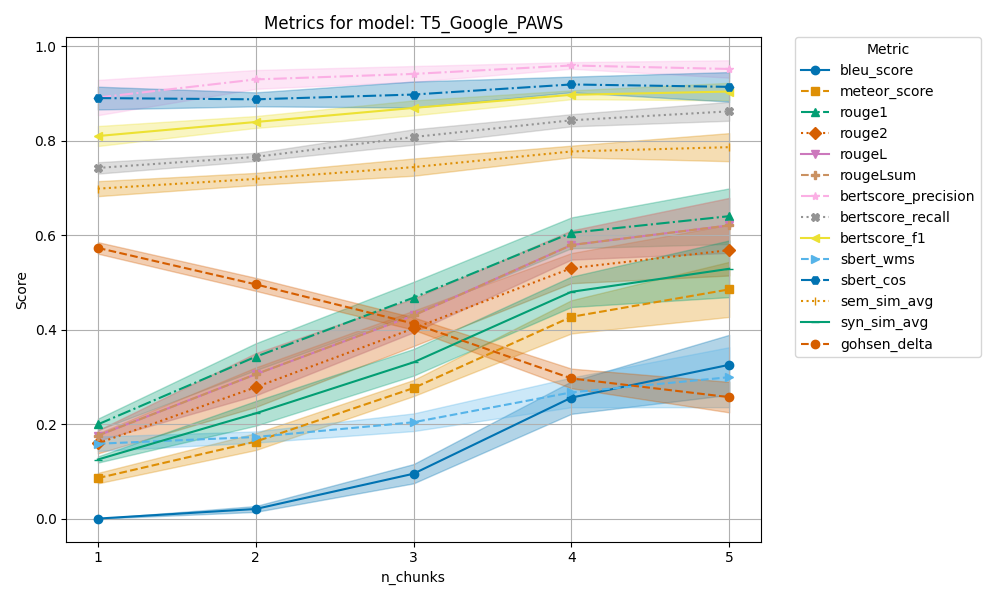
\includegraphics[width=\textwidth]{images/paraphrasing/experiments/T5_Google_PAWS_metrics_plot.png}
    \caption{Average score over different prompts (standard deviation shaded) for different paraphrasing scores for the \ac{t5} model.
    The syntactic scores rise with the number of chunks, while the semantic scores is stable.
    Consequently, the Gohsen Delta score is decreasing with the number of chunks.}
    \label{fig:abl_chunks_T5_Google_PAWS}
\end{figure}

\begin{figure}[htbp]
    \centering
    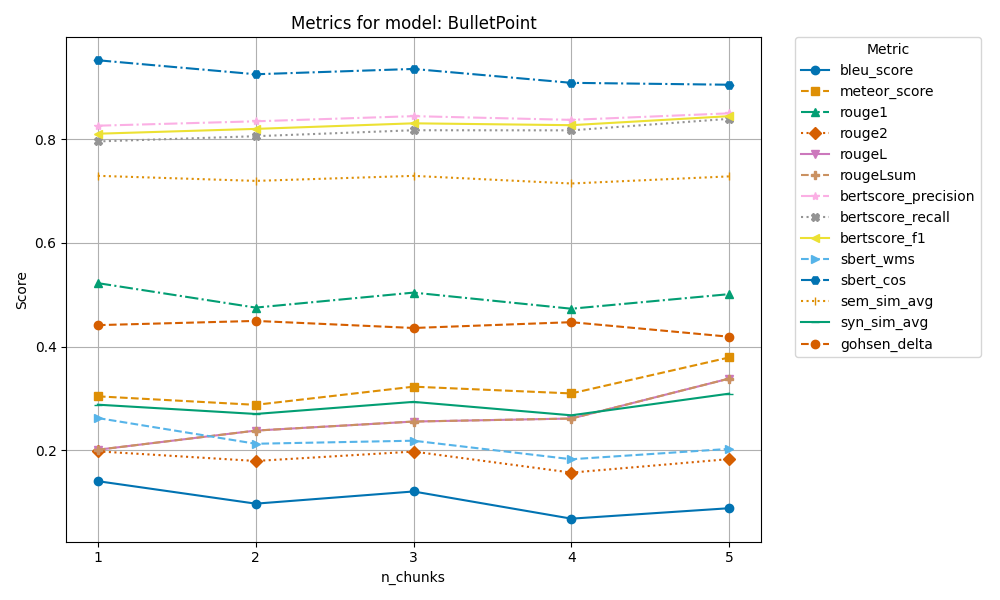
\includegraphics[width=\textwidth]{images/paraphrasing/experiments/BulletPoint_metrics_plot.png}
    \caption{Different paraphrasing scores for the BulletPoint model. 
    This model is not affected by the number of chunks.}
    \label{fig:abl_chunks_BulletPoint}
\end{figure}
    % \chapter{Conclusion \& Outlook}
\label{chap:conclusion_outlook}

    % notes
    \cite{zangerle_overview_nodate}


    % Die nächsten zwei Zeilen sind optional, sie sorgen dafür dass alles nach dem Inhalt wieder mit römischen Zahlen nummeriert wird.
    \pagenumbering{roman}
    \addtocounter{page}{10} % Dies ist die Anzahl der Seiten vor der Einleitung, muss möglicherweise angepasst werden, wenn das Inhaltsverzeichnis mehrere Seiten umfasst.

    \bibliography{
        bibliography/author_identification
    }

    \chapter*{Eidesstattliche Erklärung}

\markboth{Eidesstattliche Erklärung}{Eidesstattliche Erklärung}

Hiermit erkläre ich, \thesisauthorname, dass ich die vorliegende Arbeit mit dem Titel "\thesistitle" selbstständig 
und nur mit den nach der Prüfungsordnung der Universität Kassel zulässigen Hilfsmitteln angefertigt habe.
Die verwendete Literatur ist im Literaturverzeichnis angegeben.
Wörtlich oder sinngemäß übernommene Inhalte habe ich als solche kenntlich gemacht.

\vspace{1cm}

Kassel, \today

\begin{flushright}
  \underline{\hspace{7cm}} \\
  \thesisauthorname
\end{flushright}

\end{document}
